My theory aims to explain the gap in the treatment of domestic firms versus foreign firms. The argument will be laid out in three steps:

\begin{enumerate}
\item I argue that for FDI to have a spillover and growth enhancing effect, the domestic sector must also be healthy. Therefore, if we see the a gap in the treatment of domestic firms versus foreign firms, it must mean that the government is attracting FDI for reasons other than growth.
\item I argue that corruption (i.e. rent from foreign firms) is one such reason. If that is the case, the testable implication is that the presence of large FDI firms in corrupt countries (sectors) is associated with a large gap in the treatment of domestic versus foreign firms in those countries (sectors). At this step, the level of corruption in a country (sector) is treated as exogenous.

\item I endogenize the choice of government officials to engage in corruption by explicitly considering their utility maximization. To get a handle on the options available to the officials, I hold the political system constant by focusing on the case of Vietnam. With its provincial variation in FDI and private sector development, Vietnam serves as an insightful microcosm of the cross-national differences. I argue that, in Vietnam, whether the domestic sector is discriminated depends on the choice of the provincial official to choose between the rent of FDI firms and promotion to the central government, of which private sector development is an important criterion. 
\end{enumerate}

It is important to note that the dependent variable is \textit{not} the size of the domestic sector. First, the size of the domestic sector is a poor proxy for the government's discrimination against domestic firms in favor of foreign firms. Second, it is also a highly endogenous variable because there is definitely reverse causality between the presence of FDI (a key independent variable) and the size of the domestic sector.

\subsection{The spillover effect of FDI depends on having a strong domestic sector}

There are several channels through which spillover can happen, all of which require a strong domestic sector.
\begin{itemize}
	\item imitation:  domestic firms may reverse engineer a production or management technique \citep{Wang1992}. This requires 1) a small, surmountable technological gap \citep{Kokko1996}, and 2) backward linkage between local and foreign firms \citep{Javorcik2004}. Therefore, it is necessary to have technologically competent local firms that are able to supply inputs to foreign firms.
	\item skills acquisition: workers trained in foreign firms bring along their human capital when they move to domestic firms \citep{Djankov2000}. This presumes a healthy domestic sector that can offer competitive wages to workers. 
	\item competition: similar to arm's length trade, the presence of foreign firms put pressure on domestic firms to reduce inefficiency \citep{Glass2002}. For this mechanism to work, the domestic sector must survive instead of being squeezed out of market by foreign firms.
	\item export demonstration: foreign firms are more knowledgeable about exporting, which involves high fixed cost to set up a distribution and transport infrastructure, or learning about foreign taste and regulatory environment. Domestic firms can learn this ``export know-how'' from foreign firms \citep{Aitken1997}. This process, too, requires a strong domestic sector that is able to engage in commercial linkages with foreign firms.
\end{itemize}

In sum, the spillover effect of FDI depends on a strong domestic sector. Therefore, if a government is truly interested in FDI for its spillover and growth-enhancing effect, the government must be equally interested, if not more, in nurturing the absorptive capacity of domestic firms. Holding constant firm characteristics (size, sector, technological capacity, etc.), if we find that domestic firms receive worse treatment by the government, this can be evidence that the government is not primarily interested in the spillover effect of FDI, but potentially rent seeking.

Anticipating alternative explanations, there are reasons for countries to attract FDI other than growth and corruption, such as jobs, capital, and balance of payments. Fortunately, these alternative explanations can be controlled for. Moreover, these factors may account for the enthusiasm of the government towards FDI, but cannot fully explain the discrimination against domestic firms in favor of FDI. Indeed, many factors that are attractive to foreign firms (e.g. skilled labor force, good infrastructure, good governance) has high fixed cost but low marginal cost, and thus should be easily extended to domestic firms. Therefore, if corruption is not the government wants FDI, the domestic sector would benefit instead of being discriminated against.

\subsection{FDI and corruption (cross-nationally and cross-sectorally)}

My hypothesis that host country officials engage in corruption with foreign firms to the detriment of domestic firm is a novel contribution to the IPE literature of FDI and corruption. So far, the literature has been predominantly dominated by studies showing that a high level of corruption deters FDI \citep{Wei2000, Hakkala2008, Al-Sadig2009}. But what about firms that choose to invest in a highly corrupt environment nonetheless? One strain of the literature argues that foreign firms can help reduce corruption in host country via regulatory pressure effect, demonstration effect, and professionalization effect \citep{Kwok2006}; or via competing away the rents of the domestic firms, reducing the supply of bribes \citep{Sandholtz2003}. On the other hand, some argue that foreign firms, disadvantaged by their foreignness, have to bribe more and exacerbate corruption \citep{Hellman2002}. In all of these works, corruption between the host government and the foreign firm is conceptualized as \textit{predatory}.

My theory advances the literature by arguing that corruption between the host country and the foreign firm can be \textit{collusive}. Not all foreign firms are underdog, forced to bribe to equalize the playing field. If foreign firms enjoy regulatory privilege, they do not want to relinquish it. If foreign firms are themselves in collusion with the government, there is by definition no demonstration or professionalization effect. Indeed, foreign firms have bribed to get an upper hand in the local market\footnote{http://www.nytimes.com/2012/04/22/business/at-wal-mart-in-mexico-a-bribe-inquiry-silenced.html?pagewanted=all} or to pursue rent in protected industries \citep{Malesky2015}. In these cases, the foreign firm and the host country enter a collusive relationship, resulting in the maltreatment of domestic firms.

The sequencing of the game is as follows:
\begin{enumerate}
\item At the start of the game, the level of corruption in a country (sector) is given.\footnote{This assumption is not totally unreasonable. High level of corruption in a country may be largely the result of a political system that fails to produce accountability. Such political system is more likely to be the cause than the result of the maltreatment of domestic firms. Similarly, high level of corruption in a sector may be largely due to the nature of that sector, e.g. resource-intensive, high fixed cost leading to natural monopoy, etc. which is exogenous.}
\item  If the level of corruption is high, the government is mainly interested in FDI as a source of rent, not as a source of growth. There are several reasons why the government is interested in seeking rent from FDI firms instead of domestic firms. First, if foreign firms are more profitable than domestic firms, they have more rent to be extracted. Second, if foreign firms are larger than domestic firms, they facilitate coordination and allow corruption to be better kept secret among fewer actors. Third, if the interests of firms and the government misalign in the future, foreign firms have both the options of ``exit'' and ``voice'', whereas domestic firms only have ``voice''. The government would much prefer an exiting foreign firm to a domestic firm voicing its interest. The first and second reasons also indicate that my theory is most applicable when the entering FDI firms are large.
\item The foreign firm weighs the cost of corruption against the benefits of entering the country (sector), such as natural resource, local market, or cheap labor. If the benefit outweighs the cost, the firm enters the country (sector).\footnote{\Cref{fig:fdi_corruption} shows that among countries with a lot of FDI, the level of corruption runs the full gamut. This confirms that foreign firms often enter a country despite the cost of corruption.}
\item Since the government brings in the foreign firm for rent, not for spillover, it does not care about the development of the private sector in this country (sector). Therefore, we will see a gap in the treatment by the government of the domestic firm versus the foreign firm in this country (sector).
\end{enumerate}

The theory leads to two testable hypotheses:

\begin{quote}
Hypothesis: The presence of large FDI firms in corrupt countries is associated with a large gap in the government's treatment of domestic firms and foreign firms in those countries.
\end{quote}

\begin{quote}
Hypothesis: The presence of large FDI firms in corrupt sectors is associated with a large gap in the government's treatment of domestic firms and foreign firms in those sectors.
\end{quote}

\subsection{Endogenizing government officials' decision to engage in corruption with foreign firm}

The theory in the previous section starts with the level of corruption as a given parameter. To advance the theoretical contribution even further, it is important to endogenize the decision by the government officials to engage in corruption with foreign firm. However, ``why is a country corrupt?'' is a big and difficult question to study with a cross-national design due to an insurmountable degree of endogeneity. 

To get a handle on this question, we need to know the utility calculation of the government officials, which in turn requires knowing the options offered to the officials by the country's political economic system. Therefore, in the next step of the theory, I focus on the case of Vietnam, whose sub-national variation in FDI flow and private sector development serves as an excellent testing ground.

In addition, a cross-national study of corruption suffers from well-known conceptual and measurement issues. Conceptually, corruption means different things in different countries \citep{Rosen2010}. Empirically, even if we restrict corruption to a narrow but clear-cut definition, i.e. the act of bribery in exchange to public goods that should be equally available, it is still very difficult to measure corruption well due to sensitivity bias in surveys. Focusing on the case of Vietnam does not only keep constant the locale-dependent definition of corruption but also takes advantage of a survey list experiment conducted by \citet{Malesky2015} to accurately measure the level of corruption across provinces and sectors without sensitivity bias.

The theory is as follows. I argue that the key to the variation in provincial rent seeking of FDI is the principal-agent relationship between Vietnam's central and the provincial governments. Since most FDI projects are approved at the provincial level, it is the provincial government, not the central, that holds valuable services for sale to foreign firms. This is especially true because the implementation of central law varies widely across sub-national units in Vietnam \citep{Meyer2005}.\footnote{Vietnam's sub-national variation in implementation generalizes well to other developing countries \citep{Thun2006}} The central government, therefore, is more removed from direct contact with FDI firms and thus less likely to benefit from corruption than provincial leaders. At the same time, the central government is much more concerned with overall economic growth, which is central to the longevity of the regime \citep{Malesky2008}. Therefore, the central government is more interested in the spillover effect of FDI, which necessitates the development of a strong domestic sector as discussed.  On the other hand, each provincial leader is incentivized to free-ride on the developmental effort of other provinces and of the central to keep the entire regime stable. 

In conclusion, provincial leaders care more about private rents from FDI. In contrast, central leaders care more about the spillover effect of FDI on private sector development.

Fortunately for the central government, the principal-agent problem in this context is partially solved because monitoring is not too difficult. Indeed, the central government can observe the economic performance of the provinces and use personnel management to punish and reward provincial officials \citep{Sheng2007, Li2005}.\footnote{\citet{Shih2012} recently argue that economic performance does not matter to cadre promotion. However, they investigate all members of the Chinese Central Committee, including the central party apparatus, the army, and the central economic bureaucracy. These actors are not the important decision-makers in our theory.} Therefore, the principal-agent problem is only severe when the provincial officials are not interested in further promotion to the central government. This suggests that there will be a variation in private sector development across provinces according to the provincial officials' interest in promotion. By looking at this variation in the career interest of provincial officials, my theory contributes a fresh angle to the current literature on the relationship between decentralization and corruption, which has only postulated a one-way relationship: either decentralization increases bribery \citep{Fan2009} or reduces it \citep{Guerra2009}.

The sequencing of the game is as follows:
\begin{enumerate}
\item At the start of the game, the endowment of a province is given.\footnote{The assumption that the endowment is exogenous is reasonable. First, if it is the kind of endowment that cannot be affected by past provincial policies, e.g. natural resources, proximity to market, then it is truly exogenous. Second, even if it is the kind of endowment that can be affected by past policies, e.g. quality of the labor force, infrastructure quality, etc., it is usually good for both foreign and domestic firms. Therefore, at the start of the game, there is not yet any discrimination between foreign and domestic firms.}
\item The provincial official observes his endowment and calculates his current wealth, i.e. the return of rents from FDI firms.
\item The provincial official calculates the return of pursuing a promotion, which is a ``gamble'' with uncertainty:

the return of pursuing a promotion $=$ the return of the promotion $\times$ the probability of getting the promotion $(p)$

$p = p_0 + p_1$, with $p_0$ being the base chance of getting the promotion, and $p_1$ being the added chance if the official decides to develop the domestic sector as the central government desires.

\item The provincial official has to decide between keeping his current wealth (i.e. seek rents from FDI) or gambling (i.e. focus on private sector development to get a $p_0 + p_1$ chance of getting the promotion). Assuming that the official is risk averse, he prefers a small gamble over a large one. In this way, the base chance $p_0$ matters. If $p_0$ is small, it is highly uncertain that the official will get the promotion even with the added $p_1$. Therefore, the official is more likely to seek rent from the foreign firm instead of pursuing a promotion when the base chance $p_0$ is small. 
\end{enumerate}

Three key assumptions in the theory above deserve further examination:
\begin{enumerate}
\item Why wouldn't Vietnam's central government worry that a developed private sector may lead to social change that ultimately undermines its rule?

First, there is a large scholarship showing that authoritarian regimes are very adept at using institutions to manage regime outsiders in general and business in particular \citep{Gandhi2006, Gandhi2008, Wright2008, Le2015}. Second, if the legitimacy of the regime rests heavily on delivering economic growth, then the short-term risk of an economic downturn creating instability features much more prominently than the long-term concern with social changes. Third, it is possible to foster economic growth while restricting political freedom (e.g. Singapore). Indeed, growth can make a regime, both democratic and authoritarian, more stable, and creates room for political control \citep{Przeworski1997}.

\item Why don't provincial leaders seek rent from the domestic sector? 

First, Vietnam's private sector was very small when FDI was first allowed into Vietnam. The size and the profitability of the average domestic firm is still smaller than those of foreign firms today. Therefore, there are both fewer rents and more coordination problems if provincial officials want to seek rents from domestic firms. Second, ironically, if officials want to grow the private sector for future rent-seeking, they must promote an enabling business environment that are free from rent-seeking. In contrast, engaging in corruption with large and existing FDI firms is much more convenient. Essentially, corrupt provincial officials have shifted the cost of building a thriving domestic sectors to the home countries of FDI firms and now extract rents from the high productivity and high profitability of these firms. 

\item Is it reasonable to frame seeking rents from FDI and developing the private sector as a dichotomous choice for the provincial officials?

It is a dichotomous choice because, in exchange for bribes, provincial officials must offer some advantages over domestic firms to foreign firms. This can be lower tax rate, easier access to land, more attention to concerns of firms, etc.

\Cref{fig:fdi_bias_vietnam} provides evidence that this choice is real. The x-axis shows how helpful the province is according to domestic firms. The y-axis shows the fairness of provincial officials in treating foreign and domestic firms (as perceived by domestic firms). The graph shows that if a province is biased towards foreign firms, it will also treat domestic firms poorly (the lower-left quadrant). The relationship is even stronger among provinces with a lot of FDI (blue labels and line).
\end{enumerate}

\begin{figure}[!ht]
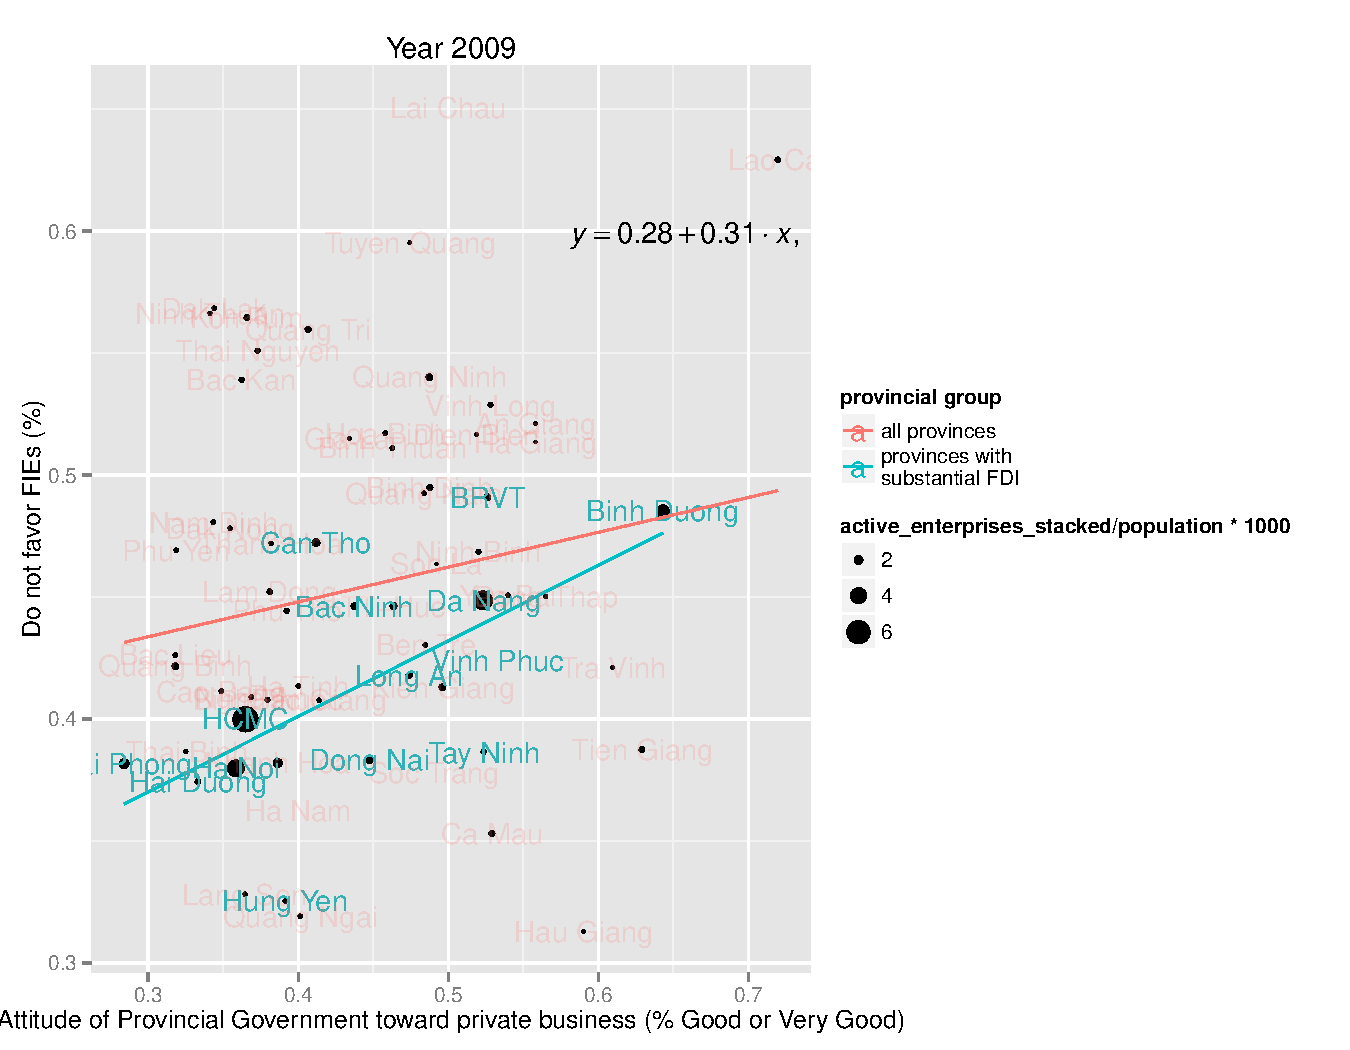
\includegraphics[width=\textwidth, height=\textheight,keepaspectratio]{../figure/FDI_bias}
\caption{The relationship between a province's FDI bias and attitude towards the private sector}
\label{fig:fdi_bias_vietnam}
\end{figure}

In sum, I propose a hypothesis about variation across Vietnam's provinces:

\begin{quote}
Hypothesis: The presence of large FDI firms in provinces whose leaders are not interested in promotion is associated with a large gap in the government's treatment of domestic and foreign firms.
\end{quote}
